\documentclass[10pt,a4paper]{article}

\usepackage[T1]{fontenc}
\usepackage{mathpazo}
\usepackage[margin=1.7cm,top=1.4cm,bottom=1.5cm,headsep=7pt]{geometry}
\usepackage{microtype}
\usepackage{booktabs,tabularx,array}
\usepackage{enumitem}
\usepackage{titlesec}
\usepackage{xcolor}
\usepackage{tikz}
\usetikzlibrary{arrows.meta,positioning}
\usepackage{caption}
\usepackage{fancyhdr}
\usepackage[hidelinks]{hyperref}
\hypersetup{
  pdftitle={When LiDAR Sees Less: A Closed-Loop Safety Assessment of Degraded Perception and HD-Map Priors for Urban Autonomous Driving},
  pdfsubject={AIE1903 AI for Autonomous Driving --- Project Proposal},
  pdfkeywords={LiDAR degradation, safety assessment, HD map, occupancy, prediction, planning, control, nuScenes}
}

\definecolor{accent}{RGB}{20,55,95}
\definecolor{warn}{RGB}{145,55,30}

\captionsetup{font=small,labelfont={bf,color=accent},skip=3pt}
\setlength{\parindent}{0pt}
\setlength{\parskip}{1.8pt}
\renewcommand{\arraystretch}{1.0}
\setlist[itemize]{leftmargin=1.05em,itemsep=1pt,topsep=2pt,parsep=0pt}
\setlist[enumerate]{leftmargin=1.35em,itemsep=1.5pt,topsep=2pt,parsep=0pt}

\titleformat{\section}{\large\bfseries\color{accent}}{\thesection}{0.55em}{}[\vspace{-3pt}{\color{accent!45}\rule{\linewidth}{0.6pt}}]
\titleformat{\subsection}{\normalsize\bfseries\color{accent!90}}{\thesubsection}{0.5em}{}
\titlespacing*{\section}{0pt}{8pt}{4pt}
\titlespacing*{\subsection}{0pt}{6pt}{2pt}

\pagestyle{fancy}
\fancyhf{}
\renewcommand{\headrulewidth}{0pt}
\fancyfoot[C]{\footnotesize\color{black!55}\thepage}

\begin{document}

\begin{center}
{\LARGE\bfseries\color{accent} When LiDAR Sees Less}\\[2pt]
{\large A Closed-Loop Safety Assessment of Degraded Perception and HD-Map Priors\\ for Urban Autonomous Driving}
\end{center}

\vspace{-4pt}
\begin{center}
{\bfseries\color{accent} Group 4}\\[3pt]
\footnotesize
\begin{tabular}{@{}l@{\hspace{2.2cm}}l@{}}
\toprule
\textbf{Teammate} & \textbf{Student ID}\\
\midrule
Gao Kai & 125090142\\
Zhou Zexuan & 125091031\\
Zhao Jiayi & 125090976\\
\bottomrule
\end{tabular}
\end{center}

\vspace{-6pt}
\section{Project Overview}

\subsection{Project title and task description}

\textbf{Project title.} \emph{When LiDAR Sees Less: A Closed-Loop Safety Assessment of Degraded Perception and HD-Map Priors for Urban Autonomous Driving.}

LiDAR is the primary geometric sensor of an urban autonomous vehicle, but its returns are not equally trustworthy in every condition. Fog and dust shorten effective range, dark or low-reflectance surfaces return few points, rain and snow perturb range, and hardware faults remove beams. An HD map supplies the complementary prior of what the road \emph{should} look like, yet it is static and can become stale after construction, temporary parking, or a changed lane topology. This project treats the two sources jointly. On nuScenes v1.0-mini, we will build a controlled degradation testbed that injects graded LiDAR faults into real sweeps, measure when safety-critical perception fails, characterise where the map prior compensates or misleads, and propagate the resulting uncertainty through a full perception--prediction--planning--control stack with a run-time safety monitor. The deliverable is a reproducible assessment, a degradation-aware fallback policy, and an evidence-based account of the operating envelope in which each source can be trusted.

\subsection{Project objectives}

\begin{enumerate}
  \item \textbf{O1 --- Degradation testbed.} Build a reproducible fault-injection pipeline on four nuScenes mini scenes (day and night) with range truncation, dropout, range noise, and combined faults.
  \item \textbf{O2 --- Safety-critical perception.} Quantify failure with a fixed-denominator safety envelope and identify the fault type and severity at which performance breaks (the ``knee'').
  \item \textbf{O3 --- Map-prior reliability.} Establish where the HD map substitutes for missing perception, where it cannot help, and where it misleads.
  \item \textbf{O4 --- Consequence propagation.} Close the loop from perception to motion, measuring whether perception deficits become collisions and what planning, control, and safety-monitor fallbacks recover, at what efficiency cost.
  \item \textbf{O5 --- Reproducible evidence.} Release a code package, demo, and report whose claims are tied to baselines, confidence intervals, and limitations.
\end{enumerate}

\subsection{Related Work and Resources}

Our design draws on four lines of work. \emph{Datasets and robustness benchmarks.} nuScenes \cite{caesar2020} provides multimodal urban data with 3D boxes, ego poses, and HD maps; Robo3D \cite{kong2023} applies controlled corruptions to LiDAR and reports 3D detection and segmentation accuracy. These benchmarks show that perception degrades under sensor faults, but they stop at perception metrics and do not test whether the degradation changes vehicle safety. \emph{Safety models.} RSS \cite{shalev2017} defines a formal safe-distance envelope from reaction time and braking limits and is widely used as a run-time monitor and minimal-risk fallback. It assumes that the state of relevant actors is known, so degraded perception requires an explicit treatment of unknown space. \emph{Planning, prediction, and control.} Frenet-frame sampling \cite{werling2010}, A* \cite{hart1968}, and MPPI \cite{williams2017} are standard components; we use them as interchangeable baselines rather than as novel algorithms. IMM \cite{blom1988} supplies the multi-model forecast and its uncertainty. \emph{Map priors.} HD maps are usually treated as static ground truth for localization and routing; their disagreement with live perception is rarely quantified as a safety variable.

The project combines these components into a single assessment: controlled LiDAR degradation, a fixed-denominator safety envelope, an A/B/C map-reliability analysis, and a closed-loop safety--efficiency evaluation. The contribution is the protocol and the evidence, not a new detector, planner, or controller. Resources are the nuScenes v1.0-mini split and devkit, numpy/scipy, and matplotlib; no pretrained model is used.

\newpage
\suppressfloats[t]
\section{Project Design}

\subsection{Research questions and hypotheses}

The design is organised around four falsifiable questions.

\begin{itemize}
  \item \textbf{RQ1 (ordering).} Which degradation first reduces safety-envelope recall and raises false-free? \emph{H1:} range truncation and dropout dominate; noise is second-order; a knee appears before the envelope is lost.
  \item \textbf{RQ2 (context).} Do night and rain scenes fail earlier at the same nominal degradation? \emph{H2:} lower density and contrast shift the knee to milder faults.
  \item \textbf{RQ3 (map).} Can the map prior compensate for degraded perception? \emph{H3:} it restores free space but cannot recover dynamic or temporary obstacles; stale cells can create false confidence.
  \item \textbf{RQ4 (closed loop).} Does a degradation-aware stack convert perception deficits into safer behaviour? \emph{H4:} it reduces collisions and gap violations at a measurable efficiency cost, whereas a blind stack that treats unknown space as free fails earlier.
\end{itemize}

Three principles guide the design: controlled degradation with fixed ground truth, so metric changes are attributable to the fault and not the frame; two evidence levels, statistical and consequential; and every claim tied to a baseline and an uncertainty interval. Rather than measuring perception accuracy or planning success in isolation, the assessment links sensor degradation to safety outcomes and to the map prior's reliability boundary.

\subsection{System architecture}

The architecture separates two questions often conflated: \emph{how much perception is lost?} and \emph{does the loss matter for motion?} Both tiers share scenes and injector, so a frame and a closed-loop run describe the same situation. The frame tier provides power over 160 keyframes; the closed-loop tier provides consequence over 20\,s segments. Figure~\ref{fig:pipeline} shows the shared data path and the two evaluation lanes.

\begin{figure}[t]
\centering
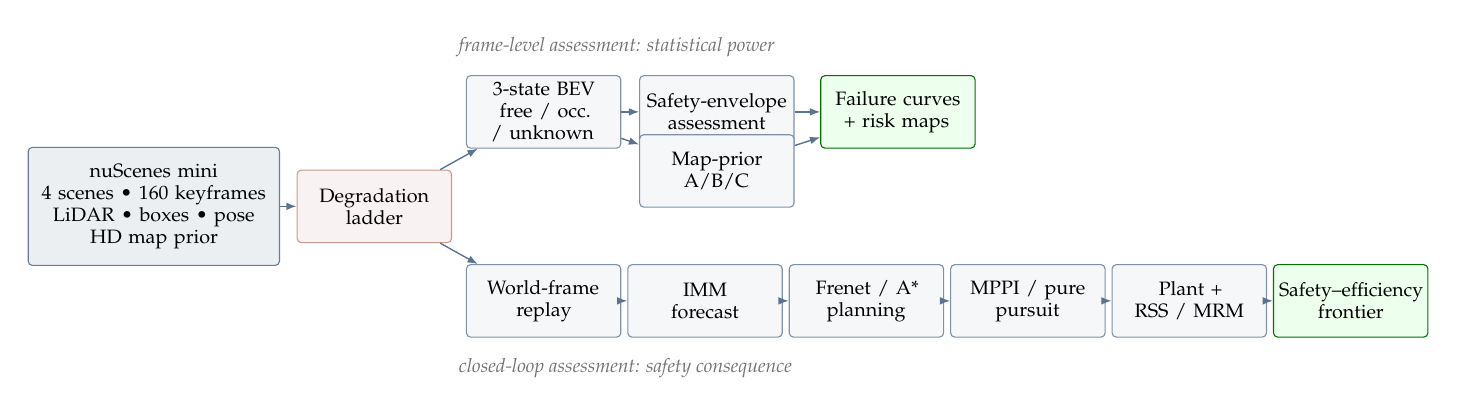
\begin{tikzpicture}[font=\scriptsize,
  box/.style={draw=accent!55, rounded corners=1.5pt, fill=accent!4, align=center,
    text width=1.82cm, minimum height=0.92cm, inner sep=2pt},
  shared/.style={draw=accent!65, rounded corners=1.5pt, fill=accent!8, align=center,
    text width=3.05cm, minimum height=1.5cm, inner sep=2pt},
  outbox/.style={draw=green!45!black, rounded corners=1.5pt, fill=green!7, align=center,
    text width=1.82cm, minimum height=0.92cm, inner sep=2pt},
  arr/.style={-{Latex[length=1.3mm]}, draw=accent!70, line width=0.5pt},
  lab/.style={font=\scriptsize\itshape, text=black!55}]

\node[shared] (src) at (0,0) {nuScenes mini\\4 scenes \textbullet\ 160 keyframes\\LiDAR \textbullet\ boxes \textbullet\ pose\\HD map prior};
\node[box, fill=warn!6, draw=warn!50] (deg) at (2.80,0) {Degradation\\ladder};
\draw[arr] (src) -- (deg);

\node[box] (bev) at (4.95,1.20) {3-state BEV\\free / occ. / unknown};
\node[box] (env) at (7.15,1.20) {Safety-envelope\\assessment};
\node[box] (map) at (7.15,0.45) {Map-prior\\A/B/C};
\node[outbox] (curves) at (9.45,1.20) {Failure curves\\+ risk maps};

\node[box] (rep) at (4.95,-1.20) {World-frame\\replay};
\node[box] (imm) at (7.00,-1.20) {IMM\\forecast};
\node[box] (plan) at (9.05,-1.20) {Frenet / A*\\planning};
\node[box] (ctrl) at (11.10,-1.20) {MPPI / pure\\pursuit};
\node[box] (plant) at (13.15,-1.20) {Plant +\\RSS / MRM};
\node[outbox] (front) at (15.20,-1.20) {Safety--efficiency\\frontier};

\draw[arr] (deg) -- (bev);
\draw[arr] (deg) -- (rep);
\draw[arr] (bev) -- (env);
\draw[arr] (bev) -- (map);
\draw[arr] (env) -- (curves);
\draw[arr] (map) -- (curves);
\draw[arr] (rep) -- (imm);
\draw[arr] (imm) -- (plan);
\draw[arr] (plan) -- (ctrl);
\draw[arr] (ctrl) -- (plant);
\draw[arr] (plant) -- (front);

\node[lab, anchor=south west] at (3.75,1.78) {frame-level assessment: statistical power};
\node[lab, anchor=north west] at (3.75,-1.80) {closed-loop assessment: safety consequence};
\end{tikzpicture}
\caption{Two-tier assessment. The same degradation ladder feeds a frame-level branch that runs the safety-envelope and map-prior assessments in parallel (top), and a closed-loop stack (bottom); both share metrics and failure cases.}
\label{fig:pipeline}
\end{figure}

\subsection{Data and degradation model}

We use nuScenes v1.0-mini keyframes from four complementary scenes: \texttt{scene-0061} (One North, day, construction), \texttt{scene-0103} (Seaport, day, pedestrians), \texttt{scene-1077} (Holland Village, night), and \texttt{scene-1094} (Holland Village, night after rain). They provide 160 synchronised keyframes with about 9.5k boxes plus 20\,Hz sweeps for closed-loop replay; the HD map combines a 0.1\,m/px drivable raster with vector lane expansion.

Table~\ref{tab:degradation} lists the ladder. Keyframes carry 3D labels and synchronised sensors and are used for the statistical assessment; sweeps are used only for closed-loop replay. Ground-truth boxes, the ego path, and the map stay fixed while only the point cloud is degraded. Stochastic levels use three seeds (five in the final sweep); truncation uses one.

\begin{table}[t]
\centering
\footnotesize
\caption{Controlled LiDAR degradation ladder. Only the point cloud changes; labels, ego path, and map are fixed.}
\label{tab:degradation}
\begin{tabularx}{\linewidth}{@{}l l X l@{}}
\toprule
\textbf{Level} & \textbf{Fault} & \textbf{Setting} & \textbf{Physical analogue}\\
\midrule
L0 & Clean & original sweep & nominal sensor\\
L1 & Range truncation & keep returns within 40 / 30 / 20 / 10\,m & fog, dust, lens contamination\\
L2 & Point dropout & remove 25 / 50 / 75\,\% of returns & low reflectance, beam failure\\
L3 & Range noise & $\sigma = 0.05 / 0.10 / 0.20$\,m along the ray & rain, snow, calibration drift\\
L4 & Combined & 20\,m truncation + 50\,\% dropout & long drive in heavy rain\\
\bottomrule
\end{tabularx}
\end{table}

\subsection{Frame-level safety assessment and map reliability}

Each sweep is rasterised into a $100\times100$\,m BEV grid at 0.2\,m with three exclusive states: \emph{free}, \emph{occupied}, and \emph{unknown}. Free space is the angular visibility profile from the ego: on each of 1440 bearings the nearest return sets the visible range, and cells beyond it are unknown. Points 0.25--12\,m above ground form the obstacle layer; a low layer (0.25--2.5\,m) prevents canopy and overhangs from sealing the road. Ground-truth boxes are rasterised only for scoring.

Safety is evaluated in an envelope built from the ego's actual 3\,s future path, 40\,m ahead and 10\,m laterally. Only actors inside can plausibly affect the ego, so the denominator is fixed across degradations. For each actor we compute $s$, $d$, and $TTC=s/v$, and count it detected when 5\,\% of its footprint is occupied. Primary metrics are envelope recall, false-free rate, urgent-miss rate among conflicts with $|d|\le3.5$\,m and $TTC\le2$\,s, and mean coverage; free-space IoU is context only. Results are stratified by range, lateral offset, class, and day/night.

The map analysis compares the map prior with live perception: \textbf{A}, map-free but occupied (stale or temporary obstacle, or map error); \textbf{B}, map-non-free but perceived free within 3\,m of road (omission or new road); \textbf{C}, map-free but unknown (occlusion or range, not a true conflict). A is attributed with ground-truth boxes; A and B accumulate in a global frame to measure persistence and ego exposure. This defines where map-only driving is safe and where fusion must trust perception.

\subsection{Closed-loop safety assessment}

The closed-loop tier replays 20\,s segments in world frame. Sweeps are transformed to world coordinates, ego-body returns removed, and the same three-state layers rebuilt around the moving ego. Annotations become agent tracks with position, heading, and speed histories. An interacting-multiple-model predictor combines constant velocity with coordinated turn over 3\,s at 0.2\,s steps, returning mode probabilities and a growing uncertainty radius.

Planning compares Frenet quintic sampling over five lateral offsets and four speed targets---with costs on clearance, unknown space, drivability, predicted collision, comfort, and progress---against risk-aware weighted A*. Control compares MPPI (192 rollouts, 2.5\,s horizon, kinematic model) with \mbox{pure pursuit}. The plant is a single-track dynamic bicycle with linear tyres, a friction circle, and a steering-rate limit, so the controller faces a mild model mismatch.

A safety monitor scans a corridor along the current lateral offset, computes an RSS-style safe distance and TTC, and runs CRUISE--CAUTION--MRM with hysteresis; MRM brakes at $2.5\,\mathrm{m/s^2}$. The key ablation is \emph{aware} versus \emph{blind}: the blind stack treats unknown space as free. A hazard injector places a virtual pedestrian or vehicle 10--40\,m ahead as a point cluster plus ground-truth box that passes through the same degradation; this creates conflicts rare in real logs and compares perception-only, map-only, fusion, and oracle variants on identical scenes.

\subsection{Evaluation protocol and expected evidence}

Four baselines anchor the analysis: B0 map-only, B1 perception-only, B2 fusion, B3 oracle. Frame metrics follow Section~2.4. Closed-loop metrics are success, collision (moving versus at-stop), minimum gap and TTC, MRM count and duration, time-to-goal, cross-track RMS, maximum lateral acceleration, and prediction RMSE. Map metrics are A/B/C area, attribution, persistence, and exposure. Stochastic conditions use scene-clustered bootstrap 95\,\% confidence intervals; grid resolution, inflation, and safety thresholds vary in a sensitivity analysis.

\textbf{Our final evidence will be} degradation--response curves with confidence intervals, a map-reliability map, and a closed-loop safety--efficiency frontier across degradation levels and stack variants. It will show which fault first breaks safety-critical perception, where the map prior can and cannot substitute, and what a degradation-aware stack buys in collisions and minimum gap per unit of lost mobility. It will \emph{not} establish real-world safety: other agents replay open-loop, faults are synthetic, and evidence covers four scenes. Claims are limited to this envelope.

\subsection{Minimum viable version, extension, and fallback}

\textbf{MVP.} The degradation ladder, three-state BEV, envelope recall and false-free curves, map A/B/C analysis, and one working closed-loop configuration (Frenet with MPPI) on all four scenes, plus a short demo.

\textbf{Extension.} Hazard injection with four baselines, the $2\times2$ planner--controller ablation, aware versus blind monitoring, all ten mini scenes (404 keyframes), a vector-map consistency layer, probabilistic occupancy with CVaR risk, Hybrid A*, and a behaviour state machine.

\textbf{Fallback.} If the dynamic plant destabilises, use a kinematic bicycle with pure pursuit. If loading is slow, use frame step two and three scenes. If conflicts remain sparse, envelope metrics and injection carry the safety claim and the closed loop is a controlled demonstration.

\subsection{Schedule and milestones}

\begin{center}
\footnotesize
\renewcommand{\arraystretch}{1.05}
\captionof{table}{Milestones from proposal submission to final delivery. Dates follow the official DL3/DL4 deadlines.}
\label{tab:schedule}\par\vspace{2pt}
\begin{tabularx}{\linewidth}{@{}l l X@{}}
\toprule
\textbf{Milestone} & \textbf{Dates} & \textbf{Deliverable and exit criterion}\\
\midrule
M1 & Nov 2--8 & Data and coordinate pipeline, degradation injector, BEV layers; unit tests pass on all four scenes.\\
M2 & Nov 9--15 & Frame-level envelope assessment and map A/B/C on all keyframes; first degradation curves with CIs.\\
M3 & Nov 16--22 & IMM prediction, Frenet/A* planning, MPPI/pure-pursuit control, RSS/MRM monitor; 20\,s runs complete.\\
M4 & Nov 23--29 & Hazard injection, $2\times2$ ablation, aware/blind comparison; sensitivity analysis.\\
M5 & Nov 30--Dec 5 & Full sweep, final figures, demo video, and draft code package.\\
M6 & Dec 6--8 & DL3 presentation and live demo; feedback recorded and triaged.\\
M7 & Dec 9--13 & Final 8--12 page report, reproducible code package, and submission.\\
\bottomrule
\end{tabularx}
\end{center}

Work proceeds weekly with metric definitions frozen after M2; later changes are recorded as sensitivity variants, not folded into the main result.

\newpage
\subsection{Risks and mitigation}

Three risks dominate. First, real conflicts are sparse: in 20\,s segments the logged ego rarely meets a safety-critical actor, so collision counts alone have low statistical power. We therefore make the safety envelope and controlled hazard injection the primary evidence and report collisions as a consequence check. Second, replay is an approximation: other agents are replayed open-loop and the nearest sweep is used as the ego moves. We bound ego deviation, report the nearest-sweep distance, and treat collisions conservatively as ego-at-fault events. Third, conclusions can depend on thresholds and grid resolution. We freeze metric definitions after M2 and report sensitivity to resolution, inflation, and RSS/unknown thresholds; if the plant proves unstable, we fall back to the kinematic bicycle and pure pursuit, which preserves the comparison.

\section{Division of Labor}

The work is organised as three workstreams around one shared evaluation contract. The core workstream owns the measurement definition and integration path, so the other two can develop against stable interfaces. Every module has a primary builder and a different reviewer; figures come from versioned scripts, never hand edits.

\begin{center}
\footnotesize
\renewcommand{\arraystretch}{1.06}
\captionof{table}{Workstreams and primary responsibilities.}
\label{tab:labor}\par\vspace{2pt}
\begin{tabularx}{\linewidth}{@{}l l X@{}}
\toprule
\textbf{Member} & \textbf{Workstream} & \textbf{Primary responsibilities and deliverables}\\
\midrule
Gao Kai & Perception and evaluation core &
Data/coordinate pipeline; degradation injector; three-state BEV; safety-envelope metrics; map A/B/C analysis; integration of both tiers; experiment orchestration; primary author of report and slides.\\
Zhou Zexuan & Prediction and planning &
Agent tracks and IMM predictor; Frenet and risk-aware A* planners; cost design; planner ablation and prediction metrics; related work and planning sections.\\
Zhao Jiayi & Control, safety, and visualisation &
Dynamic bicycle plant; MPPI and pure pursuit; RSS/MRM monitor; hazard injection; BEV and video visualisation; demo; code package, environment, and reproducibility.\\
\bottomrule
\end{tabularx}
\end{center}

The streams meet weekly: each member demonstrates a runnable artifact, reports metric deltas, and flags interface changes. The core stream maintains the figure-reproduction command and blocks merges that break it.

\begingroup
\setlength{\itemsep}{1pt}
\setlength{\parskip}{0pt}
\begin{thebibliography}{9}
\bibitem{caesar2020} H. Caesar, V. Bankiti, A. H. Lang, S. Vora, V. E. Liong, Q. Xu, A. Krishnan, Y. Pan, G. Baldan, and O. Beijbom, ``nuScenes: A multimodal dataset for autonomous driving,'' in \emph{Proc. CVPR}, 2020, pp. 11621--11631.
\bibitem{kong2023} L. Kong, Y. Liu, X. Li, R. Chen, W. Zhang, J. Ren, L. Pan, K. Chen, and Z. Liu, ``Robo3D: Towards robust and reliable 3D perception against corruptions,'' in \emph{Proc. ICCV}, 2023.
\bibitem{shalev2017} S. Shalev-Shwartz, S. Shammah, and A. Shashua, ``On a formal model of safe and scalable self-driving cars,'' \emph{arXiv:1708.06374}, 2017.
\bibitem{werling2010} M. Werling, J. Ziegler, S. Kammel, and S. Thrun, ``Optimal trajectory generation for dynamic street scenarios in a Frenet frame,'' in \emph{Proc. ICRA}, 2010, pp. 987--993.
\bibitem{hart1968} P. E. Hart, N. J. Nilsson, and B. Raphael, ``A formal basis for the heuristic determination of minimum cost paths,'' \emph{IEEE Trans. Systems Science and Cybernetics}, vol. 4, no. 2, pp. 100--107, 1968.
\bibitem{williams2017} G. Williams, A. Aldrich, and E. A. Theodorou, ``Model predictive path integral control: From theory to parallel computation,'' \emph{Journal of Guidance, Control, and Dynamics}, vol. 40, no. 2, pp. 344--357, 2017.
\bibitem{blom1988} H. A. P. Blom and Y. Bar-Shalom, ``The interacting multiple model algorithm for systems with Markovian switching coefficients,'' \emph{IEEE Trans. Automatic Control}, vol. 33, no. 8, pp. 780--783, 1988.
\end{thebibliography}
\endgroup

\end{document}
